% !TEX TS-program = xelatex
% !TEX encoding = UTF-8 Unicode

% Tennessee Technological University
% ENGR1120-021 - GSET - Summer 2021
% Tristan Hill - June 11, 2021
% Module 4 - Characters and Strings
% Lecture 4 

\documentclass[fleqn]{beamer} % for presentation (has nav buttons at bottom)

\usepackage{/home/thill/Documents/lectures/cpp_workshop/modules/cpp_lectures}

\newcommand{\MNUM}{4\hspace{2mm}} % Module number
\newcommand{\TNUM}{---\hspace{2mm}} % Topic number - single topic for now
\newcommand{\moduletitle}{Characters and Strings} % Titles and Stuff
%\newcommand{\topictitle}{---} 

\newcommand{\sectiontitleI}{The char and small integer type} % More Titles and Stuff
\newcommand{\sectiontitleII}{The ASCII Table}
\newcommand{\sectiontitleIII}{Special Characters: Escape Sequences}
\newcommand{\sectiontitleIV}{C++ Example}
\newcommand{\sectiontitleV}{Tutorial 4 -  }

\newcommand{\btVFill}{\vskip0pt plus 1filll}

\setbeamercolor{title in head/foot}{fg=TTUgold} % this needs work...

\title{GSET - Programming with Mr. Hill}
\author{Tristan Hill\vspc \hspc Tennessee Technological University \hspc}
\date{Summer 2021}

\begin{document}

\lstset{language=MATLAB,basicstyle=\ttfamily\small,showstringspaces=false}

\frame{\titlepage \center\begin{framed}\Large \textbf{Module \MNUM - \moduletitle}\end{framed} \vspace{5mm}}


% Section 0 - Outline
\frame{
	
	\large \textbf{Module \MNUM - \moduletitle} \vspace{3mm}\\
	
	\begin{itemize}
	
		\item \hyperlink{sectionI}{\sectiontitleI} \vspc % Section I
		\item \hyperlink{sectionII}{\sectiontitleII} \vspc % Section II
		\item \hyperlink{sectionIII}{\sectiontitleIII} \vspc %Section III
		\item \hyperlink{sectionIV}{\sectiontitleIV} \vspc %Section IV	
		\item \hyperlink{sectionV}{\sectiontitleV} \vspc %Section V
	
	\end{itemize}

}


% Section I
\section{\sectiontitleI}

	% Section I - Frame I
	\begin{frame}[label=sectionI,containsverbatim] \small
		\frametitle{\sectiontitleI}
		We have stored {\PN numeric} values with variables in the previous exercises.\vspace{10mm} \\ What other type of data is necessary in computer programming?
	
	\end{frame}

	% Section I - Frame II
	\begin{frame}[label=sectionI,containsverbatim] \small
	\frametitle{\sectiontitleI}
	
	
	
	\begin{lstlisting}
	
	...
	
	char c;
	
	
	
	
	...			
	
	\end{lstlisting}
	
	
	
	\btVFill
	
	%\tiny{reference: \href{https://www.cplusplus.com/doc/tutorial/operators/}{cplusplus.com} } 


	\end{frame}

% Section II
\section{\sectiontitleII}

	% Section II - Frame I

	\begin{frame}[label=sectionII] \small
	\frametitle{\sectiontitleII}
	
	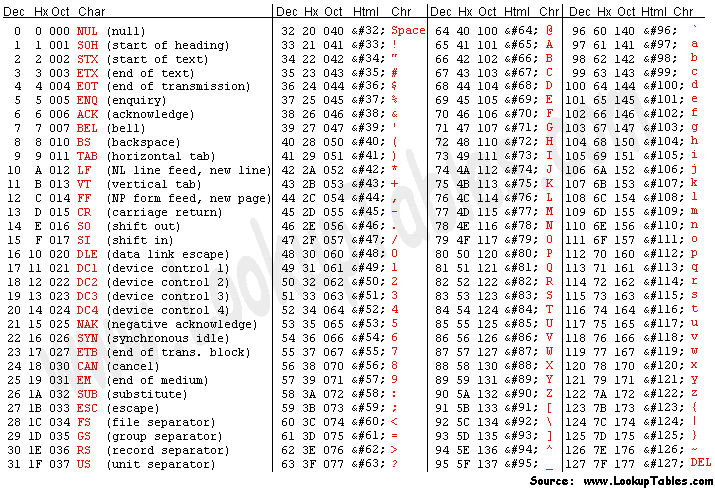
\includegraphics[scale=.35]{asciifull.png}
	
	\btVFill
	\tiny{table: \href{http://www.asciitable.com/}{asciitable.com}}
	\end{frame}
	
	% Section II - Frame II
	\begin{frame}[label=sectionII] \small
	\frametitle{\sectiontitleII}
	
	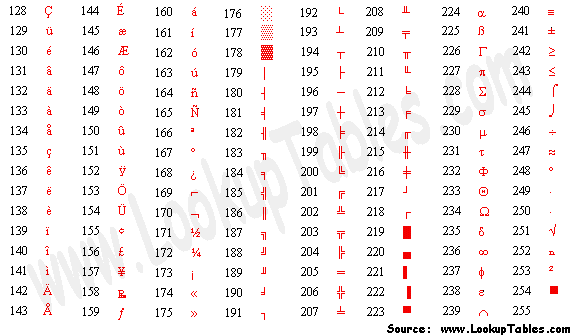
\includegraphics[scale=.35]{asciiextended.png}
	
	\btVFill
	\tiny{table: \href{http://www.asciitable.com/}{asciitable.com}}
	\end{frame}


% Section III
\section{\sectiontitleIII}

	% Section III - Frame I
	\begin{frame}[label=sectionIII] \small
		\frametitle{\sectiontitleIII}
	
		Some characters do not appear in the same way as the others.  \vspace{1mm} \\
	
			\renewcommand*{\arraystretch}{1.5}
		\begin{tabular}{c|c|c|c|c} 
			Character Name&ASCII&C++&Dec&Hex\\ \hline
			newline& NL& \textbackslash n& 10 & 0xA\\ \hline
			horiz. tab& HT& \textbackslash t & 9 & 0x9\\ \hline
			backspace& BS& \textbackslash b & 8 & 0x8\\ \hline
			carriage return & CR & \textbackslash r& 13& 0xD\\ \hline
			alert& BEL& \textbackslash a & 7 & 0x7\\ \hline
			single quote& ' & \textbackslash '& 39& 0x27\\ \hline
			double quote& "& \textbackslash "& 34& 0z22\\ \hline
	
		\end{tabular}
		
		\btVFill
		\tiny{ref: C++ Primer Plus - pg. 70}
	\end{frame}

	% Section III - Frame II
	\begin{frame}[label=sectionIII,containsverbatim] \small
	\frametitle{\sectiontitleIII}
	
		Now for some fun.
	
		\begin{lstlisting}
		
		...
		
		cout<<"\a";
		
		...
		
		
		\end{lstlisting}
	
		\btVFill
		\tiny{table: \href{http://www.asciitable.com/}{asciitable.com}}
	\end{frame}



% Section IV
\section{\sectiontitleIV}	
	% Section IV - Frame I
	\begin{frame}[label=sectionIV] \small
		\frametitle{\sectiontitleIV}    
	

		\btVFill
		%\tiny{ref: \href{some link}{some text}} 
	\end{frame}

% Section V
\section{\sectiontitleV}	
	% Section V - Frame I
	\begin{frame}[label=sectionV,containsverbatim] \small
	\frametitle{\sectiontitleV}    
	

	\end{frame}


\end{document}

